\documentclass{article}
\usepackage[T1]{fontenc}
\usepackage{geometry}
\usepackage{graphicx}
\usepackage{amsmath}
\usepackage{amssymb}

\usepackage[french]{babel}
\usepackage[utf8]{inputenc}
\usepackage[T1]{fontenc}
\usepackage{amsmath}
\usepackage{graphicx}
\usepackage{subfigure}
\usepackage{float}
\usepackage{hyperref}

%%%%%%%%%%%%%%%% Lengths %%%%%%%%%%%%%%%%
\setlength{\textwidth}{15.5cm}
\setlength{\evensidemargin}{0.5cm}
\setlength{\oddsidemargin}{0.5cm}

%%%%%%%%%%%%%%%% Variables %%%%%%%%%%%%%%%%
\def\projet{4}
\def\titre{Systèmes non-linéaires d'équations et méthode de Newton-Raphson}
\def\groupe{2}
\def\equipe{4}
\def\responsible{Margaux Lopez}
\def\secretary{Yoann Moresco}
\def\others{Yani Haouchine / Benjamin Basset}

\begin{document}

%%%%%%%%%%%%%%%% Header %%%%%%%%%%%%%%%%
\noindent\begin{minipage}{0.98\textwidth}
  \vskip 0mm
  \noindent
  { \begin{tabular}{p{7.5cm}}
      {\bfseries \sffamily
        Projet \projet} \\ 
      {\itshape \titre}
    \end{tabular}}
  \hfill 
  \fbox{\begin{tabular}{l}
      {~\hfill \bfseries \sffamily Groupe \groupe\ - Equipe \equipe \hfill~} \\[2mm] 
      Responsable : \responsible \\
      Secrétaire : \secretary \\
      Codeurs : \others
    \end{tabular}}
  \vskip 4mm ~

  ~~~\parbox{0.95\textwidth}{\small \textit{Résumé~: L'objectif de ce travail est d'étudier l'algorithme de Newton-Raphson permettant de trouver les racines d'un système non-linéaire ainsi que deux de ces applications} \sffamily }
  \vskip 1mm ~
\end{minipage}

%%%%%%%%%%%%%%%% Main part %%%%%%%%%%%%%%%%

\section{L'algorithme de Newton-Raphson}

L'algorithme de Newton-Raphson est une méthode de résolution d'équations non linéaires, mais sa convergence peut être instable si le pas de mise à jour est trop grand. Pour améliorer sa vitesse de convergence, on utilise un mécanisme de \textit{backtracking}, qui ajuste dynamiquement le pas.

\subsection{Principe du Backtracking}
\label{sec:backtracking}
Le backtracking consiste à introduire un facteur d'échelle \( \alpha \) (initialement \( \alpha = 1 \)), puis à le réduire progressivement jusqu'à obtenir une décroissance suffisante de la norme de la fonction :

\begin{equation}
U_{k+1} = U_k + \alpha \Delta U, \quad \text{avec} \quad \alpha \in [0,1].
\end{equation}

On impose la condition :

\begin{equation}
\| f(U_{k+1}) \| < \| f(U_k) \|,
\end{equation}

et on réduit \( \alpha \) selon :

\begin{equation}
\alpha \leftarrow \rho \alpha, \quad \text{où} \quad 0 < \rho < 1.
\end{equation}

Cette stratégie évite les mises à jour trop brutales et assure une meilleure convergence.

\subsection{Tests et Résultats}
\subsubsection{Test en dimension 1} 
On cherche la racine de \( f(x) = x^2 - 4 \) en partant de \( x_0 = 1 \). La solution attendue est \( x = 2 \). \\
L'algorithme avec backtracking converge correctement : 
\begin{itemize}
\item solution 2.0000000929222947 / expected solution 2.
\end{itemize}

\subsubsection{Test en dimension 2}
On résout le système :

\begin{equation}
\begin{cases}
x^2 + y^2 - 4 = 0 \\
x - y = 0
\end{cases}
\end{equation}

L'algorithme trouve bien la solution \( (\sqrt{2}, \sqrt{2}) \) : 
\begin{itemize}
\item solution [1.41421356 1.41421356] / expected solution [1.41421356 1.41421356]
\end{itemize}


\section{Calcul des points de Lagrange}

\subsection{Conception}
On sait que l'algorithme de Newton-Ralphson permet de trouver les racines d'une certaine fonction, ainsi pour résoudre notre problème il suffit de le réduire à un problème nécessitant de trouver les racines d'une telle fonction. Pour ce faire, nous créons une fonction qui représentera la somme des forces appliquées en chaque point de coordonnées (x , y). D'après le principe fondamental de la dynamique, un objet est immobile si et seulement si les forces qui lui sont appliquées se compensent, autrement dit lorsque la fonction somme des forces s'annule. Ainsi, nous avons bien réduit notre problème initial à un problème où il faut trouver la racine d'une fonction. On peut donc résoudre notre problème en utilisant Newton-Raphson. 
\subsection{Mise en oeuvre}
Ici, aucune difficulté particulière. Nos forces sont toutes facilement représentables sous forme de fonctions et elles sont toutes différentiables. On construit donc aussi facilement la matrice jacobienne.
\subsection{Résultat}

\begin{figure}[H]
    \centering
    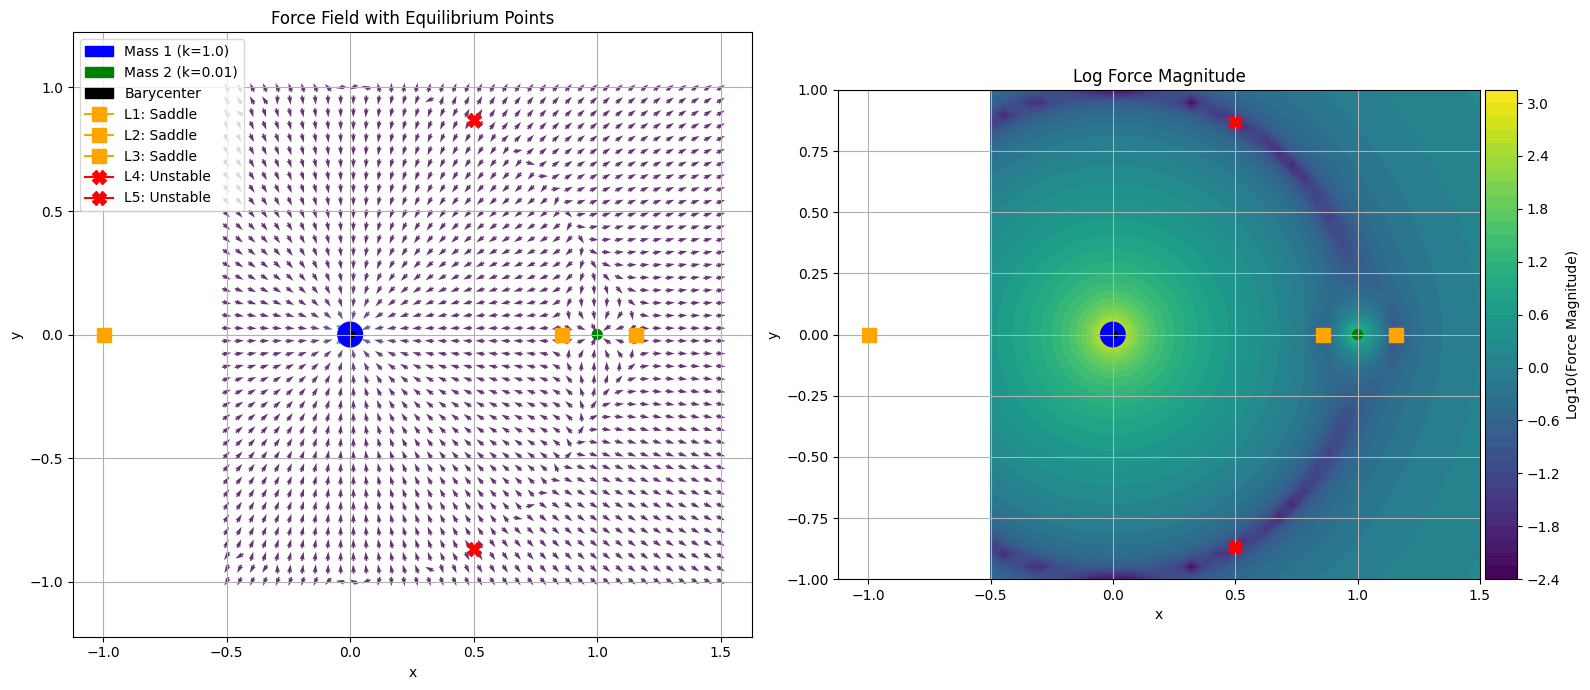
\includegraphics[width=1\linewidth]{img/Représentation_des_forces.png}
    \caption{Points de Lagrange}
    \label{fig:points_de_lagrange}
\end{figure}

On observe sur le graphique la présence de 5 points de Lagrange. Les 2 points formant un triangle isocèle avec nos astres sont stables. En effet, de petites oscillations autour d'un des deux points nous fait quand même tendre vers ce point. Les 3 autres points situées sur l'axe des deux astres sont instables. Ils sont donc difficiles à obtenir.



\section{Equilibre électrostatique}

\subsection{Principe}

La deuxième application présentée ici est l'équilibre électrostatique. Il s'agit d'un problème de physique qui met en jeu un nombre de charges, ici noté N, où l'équilibre est atteint lorsque plus aucune charge ne se déplace.

\medskip

L'idée derrière ce problème est de trouver les positions de ces N charges sur un axe gradué de -1 à 1 afin de garantir l'équilibre. Comme chaque charge porte une certaine quantité d'énergie, il est possible de quantifier l'énergie totale de ces N charges.

\noindent Cet équilibre est alors obtenu pour un extremum de l'énergie totale, ce qui correspond à un point qui annule le gradient de l'énergie totale.

\medskip

\subsection{Application de la méthode de Newton-Raphson}

C'est là que la méthode de Newton-Raphson intervient car $\nabla E(x_1, x_2, \dots, x_N) = 0$ est un système non-linéaire, où $\nabla E$ est le gradient de l'énergie.

\medskip

Par un simple développement de Taylor, on se ramène alors à l'égalité $H(E).\delta E = -\nabla E$, où H est la matrice hessienne associée à E.

\noindent Ce système se résout alors à l'aide de l'algorithme de Newton-Raphson précédemment implémenté.

\subsection{Résultats : tracés des positions d'équilibre}

\begin{figure}[H]
  \centering
  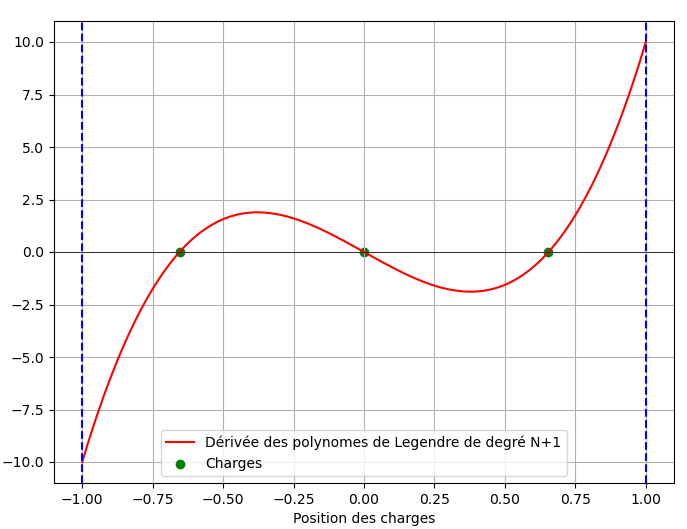
\includegraphics[height=0.4\linewidth]{img/roots_and_solutions_for_N_3.png}
  \caption{Pour N=3}
  \label{fig:f1}
\end{figure}

\bigskip

\noindent Le graphe ci-dessus présente les positions d'équilibre pour un système de 3 charges.

\begin{minipage}[c]{.5\linewidth}
  \begin{figure}[H]
    \centering
    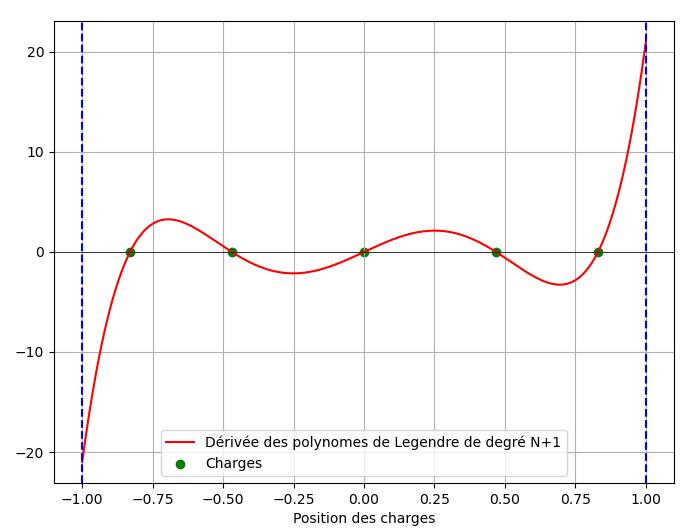
\includegraphics[height=0.75\linewidth]{img/roots_and_solutions_for_N_5.png}
    \caption{Pour N=5}
    \label{fig:f2}
  \end{figure}
\end{minipage} \hfill
\begin{minipage}[c]{.5\linewidth}
  \begin{figure}[H]
    \centering
    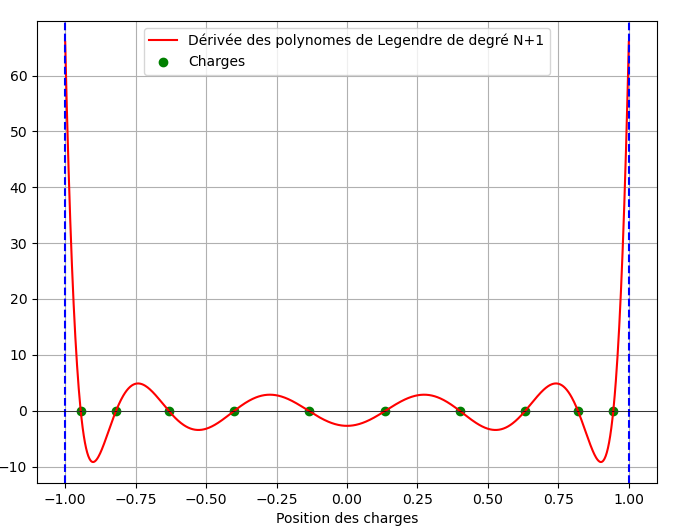
\includegraphics[height=0.75\linewidth]{img/roots_and_solutions_for_N_10.png}
    \caption{Pour N=10}
    \label{fig:f3}
  \end{figure}
\end{minipage}

\bigskip

\noindent Les graphes ci-dessus présentent les positions d'équilibre pour un système de 5 et 10 charges.

\bigskip

Les courbes obtenues sur chacun des graphes ci-dessus représentent les racines des polynômes dérivés de Legendre, obtenues à l'aide de fonctions de la bibliothèque $numpy.polynomial.legendre$.

\medskip

On constate que les racines de notre équation $\nabla E(x_1, x_2, \dots, x_N) = 0$ coïncident avec celles des polynômes dérivés de Legendre.

\subsection{Interprétation physique des solutions trouvées}

Finalement, l'étude de $H(E)$ en un point précis, caractérisé par la position des N charges, montre que la hessienne est une matrice définie négative. Cela traduit le fait qu'il s'agit d'un maximum local de la fonction E.

\medskip

Donc, la solution trouvée à $\nabla E(x_1, x_2, \dots, x_N) = 0$ est un maximum d'énergie, ce qui est cohérent avec le fait qu'un équilibre électrostatique est bien souvent instable du fait de l'intéraction permanente entre les charges.

\subsection{Impact du Backtracking sur la convergence}

Nous pouvons également étudier l'impact du backtracking développé dans la partie 1 sur la résolution du système non-linéaire associé à notre cas pratique de l'équilibre électrostatique. Pour ce faire, on observe la norme euclidienne de $\mathbb{F(U)}$ à chaque itération, où $\mathbb{F}$ est la fonction qui s'applique à $\mathbb{U}$, notre vecteur solution. Afin d'avoir un meilleur aperçu du mécanisme de convergence, nous prenons un système volontairement plus important avec N=20.

\begin{figure}[H]
  \centering
  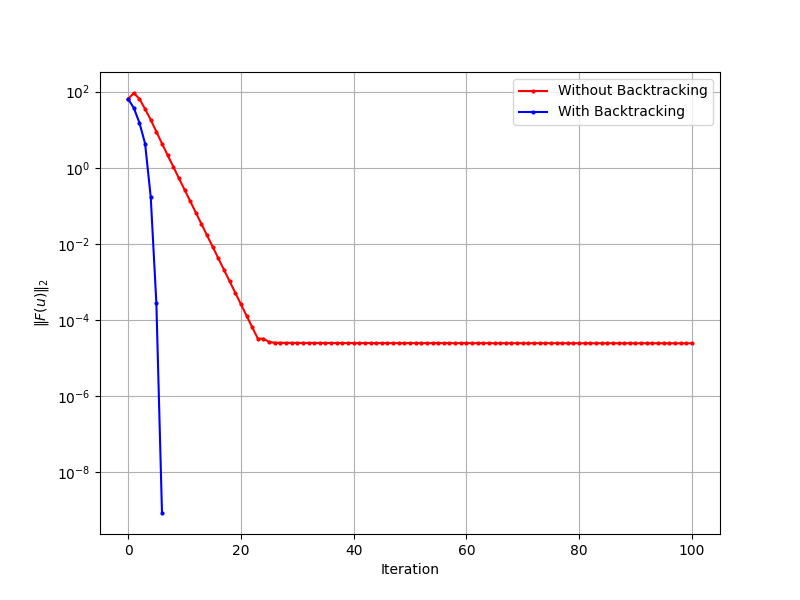
\includegraphics[height=0.5\linewidth]{img/convergence_eq_es.png}
  \caption{Convergence de la méthode Newton-Raphson pour N=20}
  \label{fig:f4}
\end{figure}

On observe sur la figure 5 que le backtracking, comme expliqué précédemment, améliore fortement la vitesse de convergence, notamment dans le cadre de système de taille importante. 
\section{Conclusion}

A travers ce projet, nous avons mis en exergue l'utilisation précieuse de l'algorithme de Newton-Raphson pour la résolution des systèmes non-linéaires d'équations. Les études des points de Lagrange et de l'équilibre électrostatique nous a également permis de mettre en avant l'intérêt du backtracking pour améliorer la vitesse de convergence de cet algorithme.

\end{document}
